\begin{figure}
\centering	
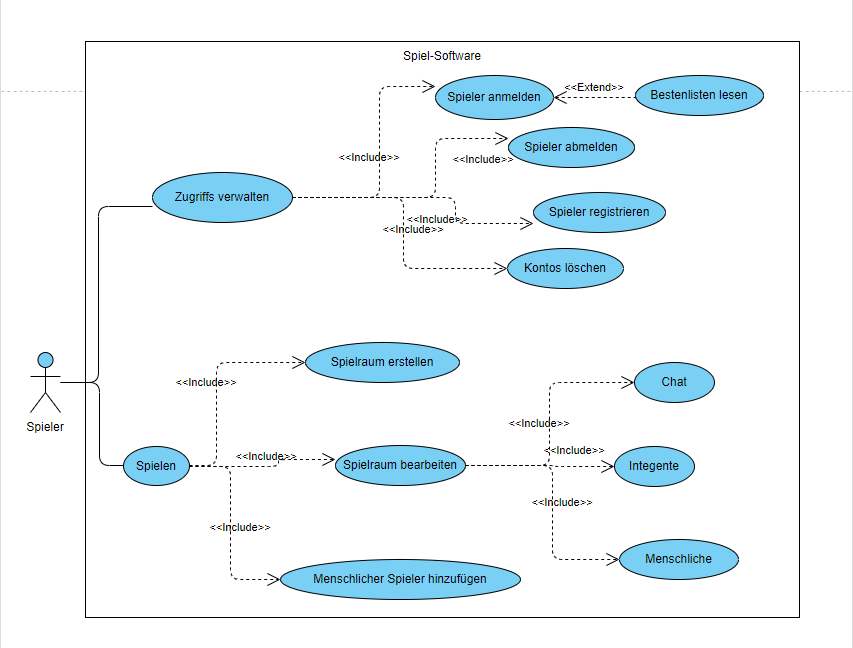
\includegraphics[width=0.9\textwidth]{img/group6.png}
\label{fig:sys}
\caption{Use Case Diagramm}
\end{figure}

\section{Systemgrenze (Use Case Diagramm)}

Die Systemgrenze wird in der Abbildung~\ref{fig:sys} dargestellt. 


\section{Beschreibungen der Anwendungsfälle}


\newcounter{uc}\setcounter{uc}{10}

\begin{description}[leftmargin=5em, style=sameline]

	\begin{lhp}{uc}{UC}{uc:zugriff}
		\item [Name:] Zugriff verwalten.
		\item [Ziel:] Zugriffsverwaltung.
		\item [Akteure:] Das System.
		\item [Vorbedingungen:] Falls vorhanden, Benutzername und Passwort. Falls nicht vorhanden, keine.
		\item [Eingabedaten:] Falls vorhanden, Benutzername \ref{daten:benutzername} und Passwort \ref{daten:passwort}. Falls nicht vorhanden, keine.
		\item [Beschreibung:] Falls schon registriert, das Spieler gibt der Benutzername und das Passwort. Falls nicht registriert, das Spieler gibt Informationen zu registrieren.  Richtigkeit vom Passwort.
		\item [Ausnahmen:] Falls der Benutzername und dass Passwort passen nicht zusammen, das System gibt dem Spieler Hinweise.
		\item [Ergebnisse und Outputdaten:] Das Spieler hat sich erfolgreich registriert oder angemeldet.
		\item [Systemfunktionen] \ref{funk:zugriff}.
	\end{lhp}

	\begin{lhp}{uc}{UC}{uc:registieren}
	    \item [Name:] Spieler registieren.
	    \item [Ziel:] Spieler registiert sich.
	    \item [Akteure:] Spieler.
	    \item [Vorbedingungen] Keine.
        \item [Eingabedaten:] Name\ref{daten:benutzername}, Passwort\ref{daten:passwort}, Email\ref{daten:email}. 
	\item [Beschreibung:] \hfill\\ \hfill\\
	1. Spieler sendet das Formular ab.\\
	2. Das System prüft ob der Benutzername schon vorhanden ist\\	
	3. Spieler erfolgreich registiert.\\			
	\item [Ausnahmen:]\hfill 
	\begin{itemize} 
		\item[] \textit{Benutzername schon vorhanden:} Das System zeigt eine Fehlermeldung an und Spieler sendet das Formular mit anderem Benutzername ab.					
		
	\end{itemize}
	\item [Ergebnisse und Outputdaten:] Spieler erfolgreich registiert.	
	\item [Systemfunktionen:] \ref{funk:zugriff}.
    \end{lhp}
	
	\begin{lhp}{uc}{UC}{uc:anmeld}
		\item [Name:] Spieler anmelden.
		\item [Ziel:] Spieler meldet sich im System an.
		\item [Akteure:] Spieler.
		\item [Vorbedingungen] Spieler ist erfolgreich angemeldet.
		\item [Eingabedaten:] Zugriffsdaten~\ref{daten:benutzername}~\ref{daten:passwort}.
		\item [Beschreibung:] \hfill\\ \hfill\\
			1. Spieler sendet das Formular ab.\\
			2. Das System prüft die Gültigkeit von Zugangsdaten.\\				
		\item [Ausnahmen:]\hfill 
	    	\begin{itemize} 
			    \item[] \textit{Passwort oder Benutzername ist falsch:} Das System zeigt eine Fehlermeldung an.					
			
		    \end{itemize}
		\item [Ergebnisse und Outputdaten:] Spieler erfolgreich angemeldet.	
		\item [Systemfunktionen:] \ref{funk:zugriff}.
	\end{lhp}
	
	\begin{lhp}{uc}{UC}{uc:namechange}
		\item [Name:] Benutzername ändern.
		\item [Ziel:] Spieler ändert seinen Benutzername.
		\item [Akteure:] Spieler.
		\item [Vorbedingungen] Spieler ist erfolgreich angemeldet.
		\item [Eingabedaten:] Zugriffsdaten~\ref{daten:benutzername}~\ref{daten:passwort}.
		\item [Beschreibung:] \hfill\\ \hfill\\
			1. Spieler sendet das Formular ab.\\
			2. Das System prüft die Gültigkeit von Zugangsdaten.\\				
		\item [Ausnahmen:]\hfill 
	    	\begin{itemize} 
			    \item[] \textit{Passwort ist falsch:} Das System zeigt eine Fehlermeldung an.					
			
		    \end{itemize}
		\item [Ergebnisse und Outputdaten:] Benutzername erfolgreich geändert.	
		\item [Systemfunktionen:] \ref{funk:acountverw}.
	\end{lhp}	
	
	\begin{lhp}{uc}{UC}{uc:pwchange}
		\item [Name:] Passwort ändern.
		\item [Ziel:] Spieler ändert sein Passwort.
		\item [Akteure:] Spieler.
		\item [Vorbedingungen] Spieler ist erfolgreich angemeldet.
		\item [Eingabedaten:] Passwort~\ref{daten:passwort}.
		\item [Beschreibung:] \hfill\\ \hfill\\
			1. Spieler sendet das Formular ab.\\
			2. Das System prüft die Gültigkeit des Passworts.\\				
		\item [Ausnahmen:]\hfill 
	    	\begin{itemize} 
			    \item[] \textit{Passwort ist falsch:} Das System zeigt eine Fehlermeldung an.					
			
		    \end{itemize}
		\item [Ergebnisse und Outputdaten:] Passwort erfolgreich geändert.	
		\item [Systemfunktionen:] \ref{funk:acountverw}.
	\end{lhp}	
	
	\begin{lhp}{uc}{UC}{uc:loeschen}
		\item [Name:] Spieler löschen.
		\item [Ziel:] Spieler entfernt seine Daten aus dem System.
		\item [Akteure:] Spieler.
		\item [Vorbedingungen] Spieler erfolgreich angemeldet.
		\item [Eingabedaten:] Passwort~\ref{daten:passwort}.
		\item [Beschreibung:] \hfill\\ \hfill\\
				1. Spieler sendet das Formular ab.\\
				2. Das System prüft die Richtigkeit des Passworts und fragt Spieler noch ein mal, ob er sich wirklich aus dem System entfernen möchte.\\
				3. Spieler bestätigt seine Intention.\\
				4. Das System entfernt alle Daten des Spielers aus der Datenbank und bewegt Spieler in den Vorraum.\\
		\item [Ausnahmen:] \hfill
			\begin{itemize} 
				\item[] \textit{Keine Löschung erwünscht:} Schritt 4 wird nicht durchgeführt.
				
			\end{itemize}
		\item [Ergebnisse und Outputdaten:] Spielerkonto wurde gelöscht.	
		\item [Systemfunktionen:] \ref{funk:zugriff}.
	\end{lhp}
   
	\begin{lhp}{uc}{UC}{uc:bestenlistesehen}
    	\item [Name:] Bestenliste lesen.
    	\item [Ziel:] Spieler liest die Bestenliste.
    	\item [Akteure:] Spieler.
    	\item [Vorbedingungen] Spieler erfolgreich angemeldet.
    	\item [Eingabedaten:] keine.
    	\item [Beschreibung:] Spieler liest die Bestenliste \ref{daten:bestenliste}.
    	\item [Ausnahmen:] keine
    	\item [Ergebnisse und Outputdaten:] Spielerkonto wurde gelöscht.	
    	\item [Systemfunktionen:] \ref{funk:bestenliste}.
    \end{lhp}

	\begin{lhp}{uc}{UC}{uc:spielen}
     	\item [Name:] Spielen.
    	\item [Ziel:] Spieler spielt.
	    \item [Akteure:] Spieler.
    	\item [Vorbedingungen] Spieler erfolgreich angemeldet.
    	\item [Eingabedaten:] keine.
    	\item [Beschreibung:] Spieler kann den Spielraum hineintreten, mit anderen Benutzern chatten und spielen	
    	\item [Ausnahmen:] keine.
    	\item [Ergebnisse und Outputdaten:] Spieler in einen Spielraum.
     	\item [Systemfunktionen:] \ref{funk:spielraum}.
    \end{lhp} 

    \begin{lhp}{uc}{UC}{uc:chat}
    	\item [Name:] Chatten.
    	\item [Ziel:] Spieler chat mit einander.
    	\item [Akteure:] Spieler.
    	\item [Vorbedingungen] Spieler erfolgreich angemeldet und steht in einem Spielraum. 
    	\item [Eingabedaten:] keine.
    	\item [Beschreibung:] Spielern chatten mit einander. 
    	\item [Ausnahmen:] keine.
    	\item [Ergebnisse und Outputdaten:] keine
    	\item [Systemfunktionen:] \ref{funk:chat}.
    \end{lhp}

    \begin{lhp}{uc}{UC}{uc:menschlicher}
    	\item [Name:] Menschlicher Spieler hinzufügen.
    	\item [Ziel:] Spieler fügt einen menschlischen Spieler zum Spielraum.
    	\item [Akteure:] Spieler.
    	\item [Vorbedingungen] Spieler steht in einem Spielraum. 
    	\item [Eingabedaten:] keine.
    	\item [Beschreibung:] Spielern fügt einen menschlichen Spieler zum Spiel
    	\item [Ausnahmen:] \hfill
    	    \begin{itemize} 
    		    \item[] \textit{Keiner aktiver Spieler gefunden:} warten für zwei Sekunden und versucht nochmal.    		
    	    \end{itemize}  
    	\item [Ergebnisse und Outputdaten:] Spieler erfolgreich gefügt.
    	\item [Systemfunktionen:] \ref{funk:chat}.
    \end{lhp}

    \begin{lhp}{uc}{UC}{uc:intelligentbots}
    	\item [Name:] Intelligente Bots hinzufügen.
    	\item [Ziel:] Spieler fügt ein Bot Spieler zum Spielraum.
    	\item [Akteure:] Spieler.
    	\item [Vorbedingungen] Spieler steht in einem Spielraum. 
      	\item [Eingabedaten:] keine.
    	\item [Beschreibung:] Spielern fügt ein Bot Spieler zum Spiel
    	\item [Ausnahmen:] keine 
    	\item [Ergebnisse und Outputdaten:] Spieler erfolgreich gefügt.
    	\item [Systemfunktionen:] \ref{funk:bots}.
    \end{lhp}


\end{description}